\documentclass[16pts]{report}
\usepackage[utf8]{inputenc}
\usepackage[T1]{fontenc}
\usepackage[francais]{babel}
\usepackage{xcolor}
\usepackage[hyphens]{url}
\usepackage[hidelinks]{hyperref}
\usepackage{amsmath}
\usepackage{graphicx}
\usepackage{geometry}
\usepackage{textcomp}
\usepackage{tabularx}
\hypersetup{hypertexnames=true}
\geometry{hmargin=2.5cm,vmargin=1.5cm}

\usepackage{float} %Option H pour les figures, utile.

%\maketitle
%\clearpage

\begin{document}
\bibliographystyle{unsrt}
\nocite{*}

\chapter{Architecture}
\label{cha:Architecture}

Nous avons choisi de regrouper chacun de nos modules dans différents fichiers.
Au cours de notre développement, nous sommes passé par plusieurs approches
où nous n'avions pas pris en compte des éléments déjà existants pouvant être
réutilisés. Voici donc le résultat final.
\begin{figure}[H]
    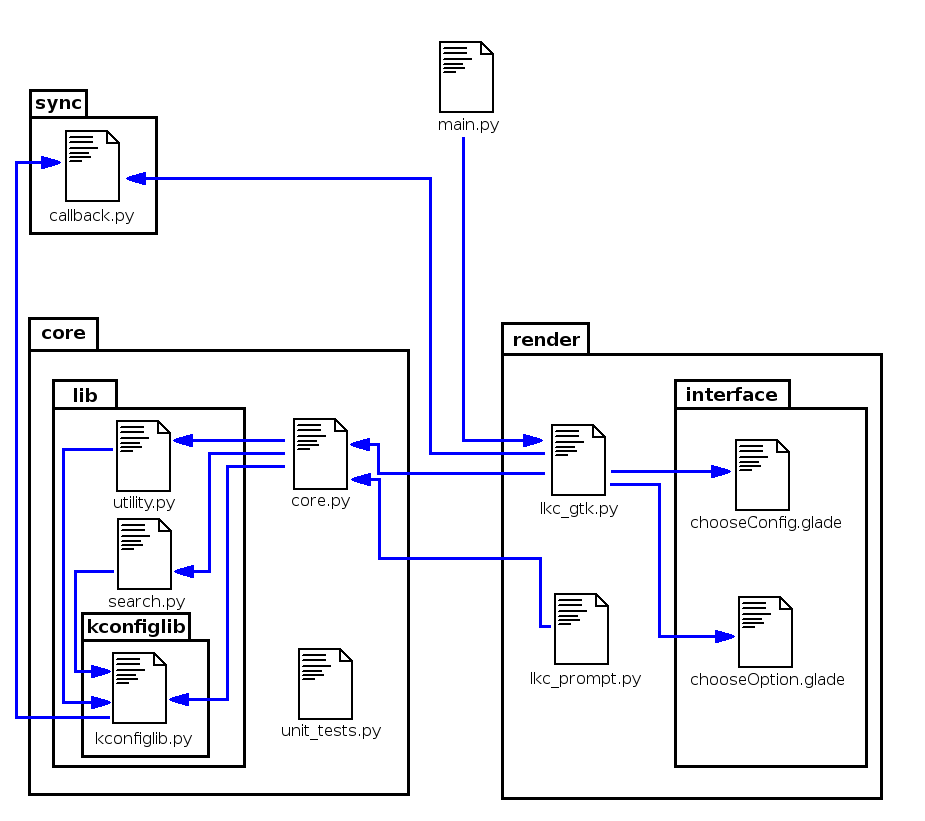
\includegraphics[scale=0.5]{illustrations/archi_add_v1.png}
    \centering
    \caption{Architecture}
    \label{fig:Arch}
\end{figure}

\section{Décomposition modulaire}
\label{sec:Décomposition modulaire}
Notre architecture se base sur le design pattern MVVM (Model View
ViewModel) une variante du concept MVC. En effet, celui-ci contient une
partie de traitement centralisée dans le module core et son affichage dans
le module render.
La différence avec le modèle MVC, c'est qu'il n'y a pas de contrôleur.  La
plupart du temps on l'utilise pour contraindre les actions de l'utilisateur
et n'avoir que des événements souhaités. Ce qui ne nous a pas paru nécessaire
dans notre projet.
L'architecture contient trois modules principaux.

    \subsection{Core}
    \label{sub:Core}
    Le module core est le "modèle" de notre architecture.
    Celui-ci représente le coeur de notre application et contient
    ses principales caractéristiques.
    Il est utilisé pour l'initialisation, le parcours et le positionnement
    de valeurs d'options d'une configuration linux générée.

    \subsection{Render}
    \label{sub:Render}
    Le module render est la "vue" de notre architecture.
    Celui-ci représente l'interface visuelle du module core. Nous utilisons
    les mécanis
    Il comporte des classes d'objets d'affichages

    \subsection{Sync}
    \label{sub:Sync}
    L'architecture choisie rend l'application maintenable, modulaire et
    indépendante du choix de l'implémentation de l'IHM. En effet, la partie
    graphique ne fait qu'afficher l'état courant de l'instance et le module
    sync permet aux bibliothèques graphiques de mettre à jour un objet, tel
    qu'une barre de chargement, pendant l'initialisation du logiciel.
    Ainsi il est aisément possible de changer, si on le souhaite, d'outil
    graphique pour QT ou autre.
    Afin de répondre à un problème de portabilité et d'extension, il est
    ou alors répondre à un de nos besoins non fonctionnel qui était de pouvoir
    lancer l'application en mode console via ncurses.



\end{document}
